\documentclass[aspectratio=1610]{beamer}
% \documentclass[handout]{beamer} % no animation version

% Theme and settings
\usetheme{Madrid}
\usecolortheme{seagull}
\usepackage{amsmath, amssymb}
\usepackage{listings}

\usepackage{xcolor}
\usepackage{tikz}
\usepackage{tikzpeople} 

% \usepackage{relsize} % for \mathlarger
\usetikzlibrary{shapes.geometric, positioning, calc, patterns, patterns.meta, backgrounds, fit, decorations.pathreplacing}

\definecolor{background}{HTML}{ffffff}
\definecolor{lightorange}{HTML}{FFE5CC}
\definecolor{highlight}{HTML}{ed7014} % orange
\colorlet{unhighlight}{background!40!gray}
\colorlet{color1}{blue}
\colorlet{color2}{red}
\colorlet{color3}{green}

\newcommand{\x}{7mm}
\newcommand{\y}{5mm}

\newcommand{\size}{\normalsize}
\newcommand{\subsize}{\tiny}

% Handle text and math mode consistent notation
\newcommand{\inmath}[1]{\relax\ifmmode \size #1 \else \size $#1$\fi}
\renewcommand{\index}[1]{\mathrm{\text{\subsize #1}}}
% \renewcommand{\index}[1]{ %
%   \ifdim \y > 2mm
%     \mathrm{\text{\normalsize #1}}%
%   \else
%     \mathrm{\text{\tiny #1}}%
%   \fi
% }

% \newcommand{\sk}[1]{\inmath{k_\index{#1}}}
% \newcommand{\PK}[1]{\inmath{K_\index{#1}}}
\newcommand{\N}[1]{\inmath{N_\index{#1}}}
\renewcommand{\S}[1]{\inmath{S_\index{#1}}}

% Generators
\newcommand{\G}[1]{\inmath{G_\index{#1}}}
\newcommand{\s}[1]{\inmath{s_\index{#1}}}
\newcommand{\sG}[2]{\inmath{\s{#1}\G{#2}}}

% Alpha, Beta, Gamma, Delta
\newcommand{\A}[1]{\inmath{\alpha_\index{#1}}}
\newcommand{\B}[2]{\inmath{\beta_\index{#1#2}}}
\newcommand{\Bprime}[2]{\inmath{\beta^\prime_\index{#1#2}}}
\newcommand{\C}[1]{\inmath{\gamma_\index{#1}}}
\newcommand{\D}{\inmath{\mathrm{\Delta}}}

% Hashes and Mappings
\newcommand{\hash}[1]{\inmath{\mathsf{h}(#1)}}
\newcommand{\sHashed}[1]{\inmath{\sigma_\index{#1}}}
\newcommand{\hashIt}[2]{\inmath{\mathsf{h}^{(#2)}(#1)}}
\newcommand{\Map}[1]{\inmath{\mathsf{Map}(#1)}}
\newcommand{\InverseMap}[1]{\inmath{\mathsf{Map}^{-1}(#1)}}


\newcommand{\at}[3]{\node at ($(#1.west) + ({#2*\x}, {-#3*\y})$)}
% \newcommand{\blocks}[4]{
%     \foreach \i in {0,...,#4}{%
%         \node at ($(#1.west) + ({(#2+\i)*\x}, {-#3*\y})$) [block=1, draw] {};
%     }
% }
\tikzset{
    p1/.style = {pattern = north east lines, pattern color = color1, opacity = 0.7, text opacity=1.0},
    p2/.style = {pattern = north west lines, pattern color = color2, fill opacity = 0.7, text opacity=1.0},
    p3/.style = {pattern = grid, pattern color = color3, opacity = 0.7, text opacity=1.0},
%     shape
    block/.style={minimum width = #1*\x, minimum height = 0.85*\y, fill=background, inner sep = 0pt, anchor=west},
%     inblock/.style={block = #1, densely dotted}, % dash pattern=on 1pt off 1pt, 
    zero_pad/.style={block = #1, fill = unhighlight, fill opacity=0.3, font=\size},
    HMAC/.style={draw, ellipse, fill = background, minimum width = \x, minimum height = \y, inner sep = 0pt, anchor = center},
    eq/.style={draw, circle, inner sep=1pt, fill=lightorange, text=black, font=\size}, %font=\bfseries\large
    arrow/.style={->, shorten <= 1pt, shorten >= 2pt},
%     line/.style={shorten <= 1pt, shorten >= 1pt},
%     dotline/.style={dotted},
%     between/.style args={#1 and #2}{at = ($(#1)!0.5!(#2)$)},
}

% % Define TikZ styles for "XOR"
% \tikzset{    
%     % shape
%     block_style/.style={minimum width = #1*\width, minimum height = \height, inner sep = 0pt, anchor = west},
%     block/.style={draw, block_style = #1},
%     inblock/.style={ultra thin, block = #1}, % dash pattern=on 1pt off 1pt, 
%     zero_pad/.style={block_style = #1, gray},
%     XOR/.style={draw, circle, minimum size=1.3*\height, 
%         append after command={
%             [shorten >=\pgflinewidth, shorten <=\pgflinewidth,]
%             (\tikzlastnode.north) edge (\tikzlastnode.south)
%             (\tikzlastnode.east) edge (\tikzlastnode.west)
%         }
%     },
%     MULT/.style={draw, circle, minimum size=1.3*\height,
%         append after command={
%             [shorten >=\pgflinewidth, shorten <=\pgflinewidth]
%             (\tikzlastnode.north west) edge (\tikzlastnode.south east)
%             (\tikzlastnode.north east) edge (\tikzlastnode.south west)
%         }
%     },
%     HMAC/.style={draw, ellipse, minimum width = \width, minimum height = \height, inner sep = 0pt, anchor = center},
%     arrow/.style={->, shorten <= 1pt, shorten >= 2pt},
%     arrowB/.style={->, shorten <= 2pt, shorten >= 4pt, color = lightgray},
%     % display
%     gray/.style={fill = gray, fill opacity=0.3},
%     green/.style={fill = green, fill opacity=0.3},
%     red/.style={fill = red, fill opacity=0.3},
%     one/.style={pattern = north east lines, pattern color = \sColor},
%     two/.style={pattern = north west lines, pattern color = \ssColor},
%     three/.style={pattern = grid, pattern color = \sssColor},
% }

\usepackage[cal=cm, scr=boondoxo, frak=pxtx]{mathalfa}

\title{Towards a Decentralized Sphinx Header Construction}
% \subtitle{Towards a Decentralized Sphinx Header Construction}
\author{Aurélien Chassagne}
\date{\today}
% \date{February 18, 2025} % \today

\begin{document}

% Title slide
\begin{frame}
\titlepage
\end{frame}

% Outline slide
% \begin{frame}{Outline}
% \tableofcontents
% \end{frame}

\begin{frame}
    \begin{enumerate}
        \item Introduction
        \begin{itemize}
            \item Motivation - Speak about importance of Privacy on the network
            \item Some Technologies: TOR vs Mixnet {\color{gray}(lot of animations)}
        \end{itemize}
        \item The problem
        \begin{itemize}
            \item Mixnet's problem (discard illegal packet at exit gateway)
            \item Our idea - Decentralization
        \end{itemize}
        \item Sphinx
        \begin{itemize}
            \item Original Sphinx {\color{gray}(lot of animations)}
            \item Our Sphinx implementation {\color{gray}(lot of animations)}
        \end{itemize}
        \item Tests and Results
        \item Conclusion and future work
    \end{enumerate}
\end{frame}
\begin{frame}{Motivation}
    \begin{center}
        -- Why privacy matters --
    \end{center}
\end{frame}
\begin{frame}{Network Privacy Technologies}
    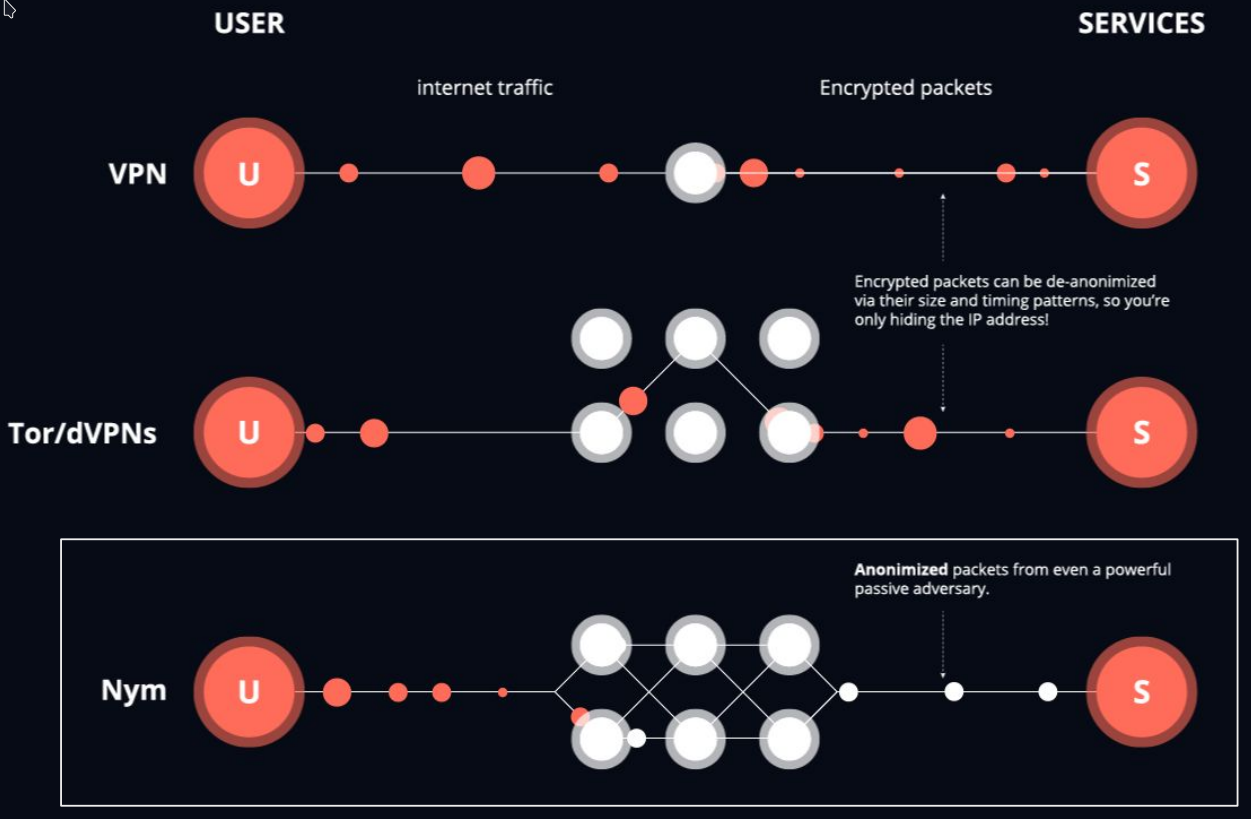
\includegraphics[width=0.8\linewidth]{networks.png}
    % VPN: Faster
    % Mixnet: More privacy
\end{frame}
\begin{frame}{The Problem - Policy enforcement at exit gateway} % Discard illegal at exit gateway

    Why \emph{policy enforcement}:
    \begin{enumerate}
        \item \textbf{Economic:} Company willing to provide different subscription plans
        \item \textbf{Political:} Enforce law regulation (i.e. reaching illegal website)
    \end{enumerate}

    \vfill

    Why at \emph{exit gateway}:
    \begin{enumerate}
        \item Privacy-friendly legitimacy verification of layered encrypted packet is tricky
        \item At exit gateway, the destination is revealed allowing easier policy enforcement
    \end{enumerate}
    
    \vfill

    Why is it a \emph{problem}:
    \begin{enumerate}
        \item Computation waste of mixnodes
    \end{enumerate}
    
    \vfill

    What we would like:
    \begin{itemize}
        \item Policy enforcement applicable at any nodes
    \end{itemize}
\end{frame}

\begin{frame}{Our Idea - Decentralized packet construction}

    % \vspace{-5mm}\hspace{-5mm}
    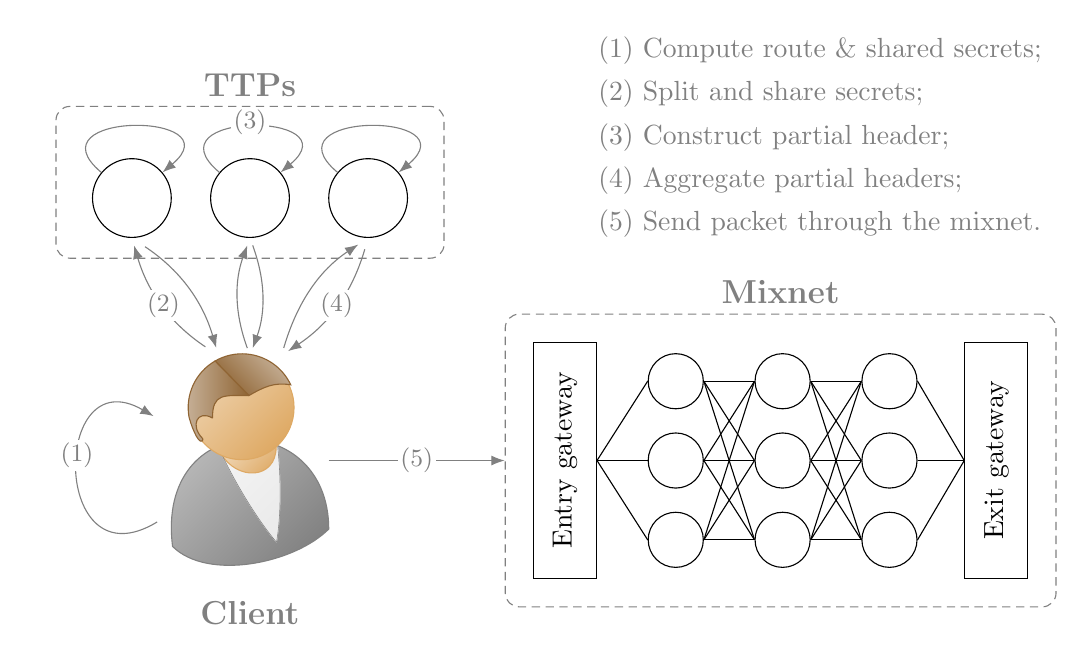
\begin{tikzpicture} 
        % Client
        \node (client) [bob, minimum size=20mm, label=below:\text{\color{gray}\large\textbf{Client}}] at (0,0) {};
        % TTPs
        \node (ttp1) [draw, circle, minimum width=10mm] at ($(client.north) + (-15mm, 20mm)$)  {};
        \node (ttp2) [draw, circle, minimum width=10mm] at ($(client.north) + (0, 20mm)$) {};
        \node (ttp3) [draw, circle, minimum width=10mm] at ($(client.north) + (15mm, 20mm)$)  {};
        \node (ttps) [draw, densely dashed, color=gray, fit={(ttp1) (ttp3)}, rounded corners=5pt, inner sep=13pt, label=above:\text{\color{gray}\large\textbf{TTPs}}, yshift=2mm] {};
        % Mixnet
        \node (entry) [draw, minimum height=30mm, minimum width=8mm] at ($(client.east) + (30mm, 0)$) {};
        \node[align=center, rotate=90] at (entry.center) {Entry gateway};
        \node (11) [draw, circle, minimum width=7mm] at ($(entry.north east) + (10mm, -5mm)$) {};
        \node (12) [draw, circle, minimum width=7mm] at ($(entry.east) + (10mm, 0)$) {};
        \node (13) [draw, circle, minimum width=7mm] at ($(entry.south east) + (10mm, 5mm)$) {};
        \node (21) [draw, circle, minimum width=7mm] at ($(11.east) + (10mm, 0)$) {};
        \node (22) [draw, circle, minimum width=7mm] at ($(12.east) + (10mm, 0)$) {};
        \node (23) [draw, circle, minimum width=7mm] at ($(13.east) + (10mm, 0)$) {};
        \node (31) [draw, circle, minimum width=7mm] at ($(21.east) + (10mm, 0)$) {};
        \node (32) [draw, circle, minimum width=7mm] at ($(22.east) + (10mm, 0)$) {};
        \node (33) [draw, circle, minimum width=7mm] at ($(23.east) + (10mm, 0)$) {};
        \node (exit) [draw, minimum height=30mm, minimum width=8mm] at ($(32.east) + (10mm, 0)$) {};
        \node[align=center, rotate=90] at (exit.center) {Exit gateway};
        \node (mixnet) [draw, densely dashed, color=gray, fit={(entry) (exit)}, rounded corners=5pt, inner sep=10pt, label=above:\text{\color{gray}\large\textbf{Mixnet}}] {};
        % links
        \draw (entry.east) -- (11.west);
        \draw (entry.east) -- (12.west);
        \draw (entry.east) -- (13.west);
        \draw (11.east) -- (21.west);
        \draw (11.east) -- (22.west);
        \draw (11.east) -- (23.west);
        \draw (12.east) -- (21.west);
        \draw (12.east) -- (22.west);
        \draw (12.east) -- (23.west);
        \draw (13.east) -- (21.west);
        \draw (13.east) -- (22.west);
        \draw (13.east) -- (23.west);
        \draw (21.east) -- (31.west);
        \draw (21.east) -- (32.west);
        \draw (21.east) -- (33.west);
        \draw (22.east) -- (31.west);
        \draw (22.east) -- (32.west);
        \draw (22.east) -- (33.west);
        \draw (23.east) -- (31.west);
        \draw (23.east) -- (32.west);
        \draw (23.east) -- (33.west);
        \draw (31.east) -- (exit.west);
        \draw (32.east) -- (exit.west);
        \draw (33.east) -- (exit.west);


        % Step 1
        \draw[-Latex, gray, loop above] (client) to[out=-150,in=150,looseness=3] node[font=\small, midway, fill=white, inner sep=1pt] {(1)} (client);
        % Step 2
        \draw[-Latex, gray, bend left=20, shorten <= 2mm, shorten >= 1mm] ($(client.north) - (4mm, 0)$) to node[font=\small, midway, fill=white, inner sep=1pt] {(2)} (ttp1.south);
        \draw[-Latex, gray, bend left=20, shorten <= 1mm, shorten >= 1mm] (client.north) to (ttp2.south);
        \draw[-Latex, gray, bend left=20, shorten <= 1mm, shorten >= 1.5mm] ($(client.north) + (4mm, 0)$) to (ttp3.south);        
        % Step 3
        \draw[-Latex, gray, loop above] (ttp1) to[out=140,in=40,looseness=4] (ttp1);
        \draw[-Latex, gray, loop above] (ttp2) to[out=140,in=40,looseness=4] node[yshift=-1.5mm, font=\small, midway, fill=white, inner sep=1pt] {(3)} (ttp2);
        \draw[-Latex, gray, loop above] (ttp3) to[out=140,in=40,looseness=4] (ttp3);
        % Step 4
        \draw[-Latex, gray, bend right=-20, shorten <= 2mm, shorten >= 1mm] (ttp1.south) to ($(client.north) - (4mm, 0)$);
        \draw[-Latex, gray, bend right=-20, shorten <= 1mm, shorten >= 1mm] (ttp2.south) to (client.north);
        \draw[-Latex, gray, bend right=-20, shorten <= 1.5mm, shorten >= 1mm] (ttp3.south) to node[font=\small, midway, fill=white, inner sep=1pt] {(4)} ($(client.north) + (4mm, 0)$);
        % Step 5
        \draw[-Latex, gray] (client.east) to node[font=\small, midway, fill=white, inner sep=1pt] {(5)} (mixnet.west);

        % Steps
        \node (step1) [gray, xshift=5mm, yshift=7mm] at (mixnet|-ttps.north) {(1) Compute route \& shared secrets;};
        \node (step2) [gray, anchor=west, yshift=-2.5mm] at (step1.south west) {(2) Split and share secrets;};
        \node (step3) [gray, anchor=west, yshift=-2.5mm] at (step2.south west) {(3) Construct partial header;};
        \node (step4) [gray, anchor=west, yshift=-2.5mm] at (step3.south west) {(4) Aggregate partial headers;};
        \node (step5) [gray, anchor=west, yshift=-2.5mm] at (step4.south west) {(5) Send packet through the mixnet.};
    \end{tikzpicture}

\end{frame}
\begin{frame}{Original Sphinx - Decryption}
    \begin{itemize}
        \item {Upper part:} Mixnet path
        \vfill
        \item {Middle part:} Packet representation
        \vfill
        \item {Lower part:} Packet processing (Fig 4)
    \end{itemize}
\end{frame}
% TODO: Top-left corner with mixnet, use the mixnode color code (rgb) instead of highlight (orange)
% TOFIX: ERROR in colors for Beta4
\begin{frame}{Original Sphinx - Encryption}
    % 1) Preprocessing: XOR truncated S
    % 2) Normal procedure (with patterns that cancel out)
    % 3) Highlight hash -> problematic to decentralized
    % 4) Our solution: ECC -> 1 Element = 1 points              %% TODO: ECC recap ?
    % 5) Final header form, highlight 7 elements

    \renewcommand{\y}{4mm}
    \renewcommand{\size}{\scriptsize}
    \renewcommand{\subsize}{\tiny}

    \begin{flushright}
    \begin{tikzpicture}

        %%%%%%%%%%%%%%%%
        %% LAST LAYER %%
        %%%%%%%%%%%%%%%%

        \node (IP) [block=1, draw] at (0,0) {\D};
        \pause

        \at{IP}{0}{1}   (s3)    [block=7, draw]     {\S{3}};
        \pause
        \at{IP}{0}{1}           [p3=1]       {};
        \at{IP}{0}{1}           [c3=1]       {};
        \at{IP}{1}{1}           [unused=6]   {};
        \node[] at (s3.center)                      {\S{3}};
        \pause

        \at{s3}{-2}{1}  (s2)    [block=7, draw]     {};
        \at{s3}{-2}{1}          [unused=3]   {};
        \at{s3}{1}{1}           [p2=4]       {};
        \at{s3}{1}{1}           [c2=4]       {};
        \node[] at (s2.center)                      {\S{2}};

        \at{s2}{-2}{1}  (s1)    [block=7, draw]     {};
        \at{s2}{-2}{1}          [unused=5]   {};
        \at{s2}{3}{1}           [p1=2]       {};
        \at{s2}{3}{1}           [c1=2]       {};
        \node[] at (s1.center)                      {\S{1}};
        \pause
        
        % XOR
        \animate{ \at{s1}{-1}{1} (xor3) [draw, circle, minimum size=0.7*\y, fill=background] {}; \draw (xor3.north) -- (xor3.south); \draw (xor3.west) -- (xor3.east); } 
        \animate{ \draw[arrow] (IP) -- (IP -| xor3) -- (xor3); }
        \animate{ \draw[shorten <= 1pt] (s3) -- (s3 -| xor3); }
        \animate{ \draw[shorten <= 1pt] (s2) -- (s2 -| xor3); }
        \animate{ \draw[shorten <= 1pt] (s1) -- (s1 -| xor3); }
        \pause
        \animate{ \node at (xor3-|IP.west)                      (B3)        [block=5, draw]     {\only<-22>{{\color{black}\B{3}{}}}}; }   
        \patterns{B3}{2}{2}{2}{4}{1}{1};
        \animate{ \draw[arrow] (xor3) -- (B3); }                                          
        \pause

        \animate{ \at{B3}{2}{3}                                 (H3B)       [block=5, draw]     {\only<-22>{{\color{black}\B{3}{}}}}; }
        \animate{ \draw[arrow] (B3) -- (H3B); }
        \patterns{H3B}{2}{2}{2}{4}{1}{1};
        \pause

        % HMAC
        \animate{ \at{B3}{-1}{1.4}                              (salt3)                             {\S{3}}; }
        \animate{ \at{B3}{1}{3}                                 (H3C)           [block=1, draw]     {\C{3}}; }
        \animate{ \draw[arrow] (B3.south -| H3C) -- (H3C); }
        \animate{ \node at (salt3-|H3C)                         (H3)            [HMAC]              {\tiny HMAC}; }
        \animate{ \draw[arrow] (salt3) -- (H3); }
        \pause

        \animate{ \at{B3}{0}{3}                                 (H3N)       [block=1, draw]     {\N{3}}; }
        \pause

        % \begin{pgfonlayer}{background}
        %     \node (box3) [fill=highlight, fill opacity=0.0, fit={(IP) (s3) (xor3) (H3B)}, rounded corners=2pt, inner sep=2pt, label=right:\rotatebox{-90}{\color{unhighlight!50}\size\textbf{Last layer}}] {};
        % \end{pgfonlayer}

        %%%%%%%%%%%%%%%%%%%
        %% MIDDLE LAYER  %%
        %%%%%%%%%%%%%%%%%%%

        \animate{ \at{H3N}{0}{1.5}            (S2)        [block=7, draw]     {{\color{black}\S{2}}}; }      
        \patternB{S2}{1}{7}                    
        \animate{ \at{S2}{-1}{1}              (xor2)      [draw, circle, minimum size=0.7*\y, fill=background] {}; \draw (xor2.north) -- (xor2.south); \draw (xor2.west) -- (xor2.east); }
        \animate{ \draw[arrow] (H3N) -- (H3N -| xor2) -- (xor2); }
        \animate{ \draw[shorten <= 1pt] (S2) -- (S2 -| xor2); }
        \pause  
        \animate{ \node at (xor2-|S2.west)                      (B2)        [block=5, draw]     {\only<-21>{{\color{black}\B{2}{}}}}; }
        \animate{ \draw[arrow] (xor2) -- (B2); }
        \patterns{B2}{4}{2}{1}{3}{3}{1}
        \at{B2}{5}{0}                                           (zero2)     [zero_pad=2]        {0};
        \only<\t>{\patternB{s2}{4}{4}}
        \only<\t>{\patternB{B3}{2}{4}}
        \only<\t>{\patternB{H3B}{2}{4}}
        \only<\t>{\patternB{S2}{1}{7}}
        \only<\t>{\patternB{B2}{1}{3}}
        \pause
        
        \animate{ \at{B2}{2}{3}                                 (H2B)       [block=5, draw]     {\only<-21>{{\color{black}\B{2}{}}}}; }
        \animate{ \draw[arrow] (B2) -- (H2B); }
        \patterns{H2B}{4}{2}{1}{3}{3}{1}
        \pause

        % HMAC
        \animate{ \at{B2}{-1}{1.4}                              (salt2)                         {\S{2}}; }
        \animate{ \at{B2}{1}{3}                                 (H2C)       [block=1, draw]     {\C{2}}; } 
        \animate{ \draw[arrow] (B2.south -| H2C) -- (H2C); }
        \animate{ \node at (salt2-|H2C)                         (H2)        [HMAC]              {\tiny HMAC}; }
        \animate{ \draw[arrow] (salt2) -- (H2); }
        \pause

        \animate{ \at{B2}{0}{3}                                 (H2N)       [block=1, draw]     {\N{2}}; }
        \pause

        % \begin{pgfonlayer}{background}
        %     \node (box2) [fill=highlight, fill opacity=0.1, fit={(S2) (xor2) (H2B)}, rounded corners=2pt, inner sep=2pt, label=right:\rotatebox{-90}{\color{highlight!50}\size\textbf{Middle layer}}] {};
        % \end{pgfonlayer}

        %%%%%%%%%%%%%%%%%%
        %% FIRST LAYER  %%
        %%%%%%%%%%%%%%%%%%

        \animate{ \at{H2N}{0}{1.5}            (S1)        [block=7, draw]     {{\color{black}\S{1}}}; }     
        \patternA{S1}{1}{7}                    
        \animate{ \at{S1}{-1}{1}              (xor1)      [draw, circle, minimum size=0.7*\y, fill=background] {}; \draw (xor1.north) -- (xor1.south); \draw (xor1.west) -- (xor1.east); } 
        \animate{ \draw[arrow] (H2N) -- (H2N -| xor1) -- (xor1); }
        \animate{ \draw[shorten <= 1pt] (S1) -- (S1 -| xor1); }
        \pause
        \animate{ \node at (xor1-|S1.west)                      (B1)        [block=5, draw]     {\only<-20>{{\color{black}\B{1}{}}}}; } 
        \animate{ \draw[arrow] (xor1) -- (B1); }   
        \patterns{B1}{1}{5}{3}{3}{5}{1};
        \at{B1}{5}{0}                                           (zero1)     [zero_pad=2]        {0}; 
        \only<\t>{\patternB{s1}{6}{2}}
        \only<\t>{\patternB{B3}{2}{2}}
        \only<\t>{\patternB{H3B}{2}{2}}
        \only<\t>{\patternB{B2}{4}{2}}
        \only<\t>{\patternA{H2B}{4}{2}}
        \only<\t>{\patternA{S1}{1}{7}}
        \only<\t>{\patternA{B1}{1}{5}}
        \pause
        
        \animate{ \at{B1}{2}{3}                                 (H1B)       [block=5, draw]     {\only<-20>{{\color{black}\B{1}{}}}}; } 
        \animate{ \draw[arrow] (B1) -- (H1B); }
        \patterns{H1B}{1}{5}{3}{3}{5}{1}
        \pause

        % HMAC
        \animate{ \at{B1}{-1}{1.4}                              (salt1)                         {\S{1}}; }
        \animate{ \at{B1}{1}{3}                                 (H1C)       [block=1, draw]     {\C{1}}; } 
        \animate{ \draw[arrow] (B1.south -| H1C) -- (H1C); }
        \animate{ \node at (salt1-|H1C)                         (H1)        [HMAC]              {\tiny HMAC}; }
        \animate{ \draw[arrow] (salt1) -- (H1); }
        \pause

        \animate{ \at{B1}{0}{3}                                 (H1N)       [block=1, draw]     {\N{1}}; } 
        \pause

        \animate{ \node at (salt3-|H3C)            [HMAC]              {\tiny HMAC}; }
        \animate{ \node at (salt2-|H2C)            [HMAC]              {\tiny HMAC}; }
        \animate{ \node at (salt1-|H1C)            [HMAC]              {\tiny HMAC}; }
        \pause

        \only<\t>{  \animate{\at{H2N}{0}{0} [block=1, draw] {\N{2}};} }
        \only<\t>{  \animate{\at{H2C}{0}{0} [block=1, draw] {\C{2}};} }
        \only<\t>{  \animate{\at{B1}{0.5}{0} {\N{2}};} }
        \only<\t>{  \animate{\at{B1}{1.5}{0} {\C{2}};} }
                    \animate{\at{H1B}{0.5}{0} {\N{2}};}
                    \animate{\at{H1B}{1.5}{0} {\C{2}};}
        \pause
        \only<\t>{  \animate{\at{H3N}{0}{0} [block=1, draw] {\N{3}};} }
        \only<\t>{  \animate{\at{H3C}{0}{0} [block=1, draw] {\C{3}};} }
        \only<\t>{  \animate{\at{B2}{0.5}{0} {\N{3}};} }
        \only<\t>{  \animate{\at{B2}{1.5}{0} {\C{3}};} }
        \only<\t>{  \animate{\at{H2B}{0.5}{0} {\N{3}};} }
        \only<\t>{  \animate{\at{H2B}{1.5}{0} {\C{3}};} }
        \only<\t>{  \animate{\at{B1}{2.5}{0} {\N{3}};} }
        \only<\t>{  \animate{\at{B1}{3.5}{0} {\C{3}};} }
                    \animate{\at{H1B}{2.5}{0} {\N{3}};}
                    \animate{\at{H1B}{3.5}{0} {\C{3}};}
        \pause
        \only<\t>{  \animate{\at{B3}{0.5}{0} {\D};} }
        \only<\t>{  \animate{\at{H3B}{0.5}{0} {\D};} }
        \only<\t>{  \animate{\at{B2}{2.5}{0} {\D};} }
        \only<\t>{  \animate{\at{H2B}{2.5}{0} {\D};} }
        \only<\t>{  \animate{\at{B1}{4.5}{0} {\D};} }
                    \animate{\at{H1B}{4.5}{0} {\D};}
        \pause

        % \begin{pgfonlayer}{background}
        %     \node (box1) [fill=highlight, fill opacity=0.0, fit={(S1) (xor1) (H1B)}, rounded corners=2pt, inner sep=2pt, label=right:\rotatebox{-90}{\color{unhighlight!50}\size\textbf{First layer}}] {};
        % \end{pgfonlayer}

        %%%%%%%%%%%
        %% OTHER %%
        %%%%%%%%%%% 

        % \begin{pgfonlayer}{background}
        %     % Separators
        %     \node (mid32) at ($(H3N)!0.5!(S2)$) {}; \draw (mid32-|{$(box2.west)-(2mm,0)$}) -- (mid32-|{$(box2.east)+(4mm,0)$}) [densely dotted, color=unhighlight!50, line width=1pt];
        %     \node (mid21) at ($(H2N)!0.5!(S1)$) {}; \draw (mid21-|{$(box2.west)-(2mm,0)$}) -- (mid21-|{$(box2.east)+(4mm,0)$}) [densely dotted, color=unhighlight!50, line width=1pt];
        % \end{pgfonlayer}
    \end{tikzpicture}
    \end{flushright}
\end{frame}
\begin{frame}{\color{red} ECC slide}
    {\color{red} Is it neeeded ? Generator ?}
\end{frame}
% \onslide<1-9> {...}       => Without replacement (will be masked if not displayed)
% \only<3> {...}            => With replacement (overwritte)
% \pause

\begin{frame}{Our decentralized Sphinx construction}

    % 1) cut in chunks 
    % 2) 1 indep generator by chunk
    % 3) XOR -> ECC addition and substraction
    % 4) HMAC -> integrity check

    \renewcommand{\x}{7mm}
    \renewcommand{\y}{4mm} 
    \renewcommand{\size}{\scriptsize}
    \renewcommand{\subsize}{\tiny}

    \begin{flushright}
    \begin{tikzpicture}
        \size
        \node at (140pt, -204pt) {}; % for common alignement
        
        \updatebeamerpauses{1}
        \only<1-2>{%%%%%%%%%%%%%%%%
%% LAST LAYER %%
%%%%%%%%%%%%%%%%

\node (IP) [block=1, draw] at (0,0) {\D};

\at{IP}{0}{1}   (s3)    [block=7, draw]     {\S{3}{}};
\at{IP}{0}{1}           [p3=1]       {};
\at{IP}{0}{1}           [c3=1]       {};
\at{IP}{1}{1}           [unused=6]   {};
\node[] at (s3.center)                      {\S{3}{}};

\at{s3}{-2}{1}  (s2)    [block=7, draw]     {};
\at{s3}{-2}{1}          [unused=3]   {};
\at{s3}{1}{1}           [p2=4]       {};
\at{s3}{1}{1}           [c2=4]       {};
\node[] at (s2.center)                      {\S{2}{}};

\at{s2}{-2}{1}  (s1)    [block=7, draw]     {};
\at{s2}{-2}{1}          [unused=5]   {};
\at{s2}{3}{1}           [p1=2]       {};
\at{s2}{3}{1}           [c1=2]       {};
\node[] at (s1.center)                      {\S{1}{}};

% XOR
\at{s1}{-1}{1} (xor3) [draw, circle, minimum size=0.7*\y, fill=background] {}; \draw (xor3.north) -- (xor3.south); \draw (xor3.west) -- (xor3.east); 
\draw[arrow] (IP) -- (IP -| xor3) -- (xor3);
\draw[shorten <= 1pt] (s3) -- (s3 -| xor3);
\draw[shorten <= 1pt] (s2) -- (s2 -| xor3);
\draw[shorten <= 1pt] (s1) -- (s1 -| xor3);
\node at (xor3-|IP.west)                      (B3)        [block=5, draw]     {\B{3}{}};   
\patterns{B3}{2}{2}{2}{4}{1}{1}
\draw[arrow] (xor3) -- (B3);                                          

\at{B3}{2}{3}                                 (H3B)       [block=5, draw]     {\B{3}{}};
\draw[arrow] (B3) -- (H3B);
\patterns{H3B}{2}{2}{2}{4}{1}{1}

% HMAC
\at{B3}{-1}{1.4}                              (salt3)                             {\S{3}{}};
\at{B3}{1}{3}                                 (H3C)           [block=1, draw]     {\C{3}};
\draw[arrow] (B3.south -| H3C) -- (H3C);
\node at (salt3-|H3C)                         (H3)            [HMAC]              {\tiny HMAC};
\draw[arrow] (salt3) -- (H3);

\at{B3}{0}{3}                                 (H3N)       [block=1, draw]     {\N{3}};

%%%%%%%%%%%%%%%%%%%
%% MIDDLE LAYER  %%
%%%%%%%%%%%%%%%%%%%

\at{H3N}{0}{1}              (S2)        [block=7, draw]     {{\color{black}\S{2}{}}};      
\patternB{S2}{1}{7}                    
\at{S2}{-1}{1}              (xor2)      [draw, circle, minimum size=0.7*\y, fill=background] {}; \draw (xor2.north) -- (xor2.south); \draw (xor2.west) -- (xor2.east);
\draw[arrow] (H3N) -- (H3N -| xor2) -- (xor2);
\draw[shorten <= 1pt] (S2) -- (S2 -| xor2);
\node at (xor2-|S2.west)                      (B2)        [block=5, draw]     {\B{2}{}};
\draw[arrow] (xor2) -- (B2);
\patterns{B2}{4}{2}{1}{3}{3}{1}
\at{B2}{5}{0}                                           (zero2)     [zero_pad=2]        {0};

\at{B2}{2}{3}                                 (H2B)       [block=5, draw]     {\B{2}{}};
\draw[arrow] (B2) -- (H2B);
\patterns{H2B}{4}{2}{1}{3}{3}{1}

% HMAC
\at{B2}{-1}{1.4}                              (salt2)                         {\S{2}{}};
\at{B2}{1}{3}                                 (H2C)       [block=1, draw]     {\C{2}}; 
\draw[arrow] (B2.south -| H2C) -- (H2C);
\node at (salt2-|H2C)                         (H2)        [HMAC]              {\tiny HMAC};
\draw[arrow] (salt2) -- (H2);

\at{B2}{0}{3}                                 (H2N)       [block=1, draw]     {\N{2}};

%%%%%%%%%%%%%%%%%%
%% FIRST LAYER  %%
%%%%%%%%%%%%%%%%%%

\at{H2N}{0}{1}              (S1)        [block=7, draw]     {{\color{black}\S{1}{}}};     
\patternA{S1}{1}{7}                    
\at{S1}{-1}{1}              (xor1)      [draw, circle, minimum size=0.7*\y, fill=background] {}; \draw (xor1.north) -- (xor1.south); \draw (xor1.west) -- (xor1.east); 
\draw[arrow] (H2N) -- (H2N -| xor1) -- (xor1);
\draw[shorten <= 1pt] (S1) -- (S1 -| xor1);
\node at (xor1-|S1.west)                      (B1)        [block=5, draw]     {\B{1}{}}; 
\draw[arrow] (xor1) -- (B1);   
\patterns{B1}{1}{5}{3}{3}{5}{1}
\at{B1}{5}{0}                                           (zero1)     [zero_pad=2]        {0}; 

\at{B1}{2}{3}                                 (H1B)       [block=5, draw]     {}; 
\draw[arrow] (B1) -- (H1B);
\patterns{H1B}{1}{5}{3}{3}{5}{1}

% HMAC
\at{B1}{-1}{1.4}                              (salt1)                         {\S{1}{}};
\at{B1}{1}{3}                                 (H1C)       [block=1, draw]     {\C{1}}; 
\draw[arrow] (B1.south -| H1C) -- (H1C);
\node at (salt1-|H1C)                         (H1)        [HMAC]              {\tiny HMAC};
\draw[arrow] (salt1) -- (H1);

\at{B1}{0}{3}                                 (H1N)       [block=1, draw]     {\N{1}}; 

%%%%%%%%%%%%%%%%%%%%%%%%%%%%%%%%%%%%%%%%%%%%%%%%%%%%%%%%%%%%%%%%%%%%%%%%%%%%%%%%%%%%%%%%%%%%%%

\slide{0}{
    \at{H1B}{0.5}{0} {\N{2}};
    \at{H1B}{1.5}{0} {\C{2}};
    \at{H1B}{2.5}{0} {\N{3}};
    \at{H1B}{3.5}{0} {\C{3}};
    \at{H1B}{4.5}{0} {\D};
}
\incrementAnimation
\slide{1}{
    \at{H1B}{0}{0} [block=1, draw] {\N{2}};
    \at{H1B}{1}{0} [block=1, draw] {\C{2}};
    \at{H1B}{2}{0} [block=1, draw] {\N{3}};
    \at{H1B}{3}{0} [block=1, draw] {\C{3}};
    \at{H1B}{4}{0} [block=1, draw] {\D};
}}
        \updatebeamerpauses{3}
        \only<3>{\input{slides/6_solution/2_chunks.tex}}
        \updatebeamerpauses{4}
        \only<4-7>{
\newcommand{\sGrainbow}[2]{\inmath{{\color{black}s_\index{#1}}{\color{rainbow#2}G_\index{#2}}}}

%%%%%%%%%%%%%%%%%%%
%% PREPROCESSING %%
%%%%%%%%%%%%%%%%%%%

\node (IP) [block=1, draw] at (0,0) {\D};

\slide{0}{
    \block{IP}{0}{1}   (s3)    {\S{3}{1}};
    \block{s3}{1}{0}           {\S{3}{2}};
    \block{s3}{2}{0}           {\S{3}{3}};
    \block{s3}{3}{0}           {\S{3}{4}};
    \block{s3}{4}{0}           {\S{3}{5}};
    \block{s3}{5}{0}           {\S{3}{6}};
    \block{s3}{6}{0}           {\S{3}{7}};
}
\slide{1}{
    \block{s3}{-2}{1}  (s2)    {\S{2}{1}};
    \block{s2}{1}{0}           {\S{2}{2}};
    \block{s2}{2}{0}           {\S{2}{3}};
    \block{s2}{3}{0}           {\S{2}{4}};
    \block{s2}{4}{0}           {\S{2}{5}};
    \block{s2}{5}{0}           {\S{2}{6}};
    \block{s2}{6}{0}           {\S{2}{7}};
}
\slide{1}{
    \block{s2}{-2}{1}  (s1)    {\S{1}{1}};
    \block{s1}{1}{0}           {\S{1}{2}};
    \block{s1}{2}{0}           {\S{1}{3}};
    \block{s1}{3}{0}           {\S{1}{4}};
    \block{s1}{4}{0}           {\S{1}{5}};
    \block{s1}{5}{0}           {\S{1}{6}};
    \block{s1}{6}{0}           {\S{1}{7}};
}

\block{IP}{0}{4}       (B31)      {\B{3}{1}};
\block{B31}{1}{0}      (B32)      {\B{3}{2}};
\block{B31}{2}{0}      (B33)      {\B{3}{3}};
\block{B31}{3}{0}      (B34)      {\B{3}{4}};
\block{B31}{4}{0}      (B35)      {\B{3}{5}};

\block{B31}{0}{3}      (H3N)       {\N{3}}; 
\block{H3N}{1}{0}      (H3C)       {\C{3}}; 
\block{H3N}{2}{0}      (H3B1)      {\B{3}{1}};
\block{H3N}{3}{0}      (H3B2)      {\B{3}{2}};
\block{H3N}{4}{0}      (H3B3)      {\B{3}{3}};
\block{H3N}{5}{0}      (H3B4)      {\B{3}{4}};
\block{H3N}{6}{0}      (H3B5)      {\B{3}{5}};

% XOR
\at{B31}{-5}{0} (xor3) [draw, circle, minimum size=0.7*\y, fill=background] {}; \draw (xor3.north) -- (xor3.south); \draw (xor3.west) -- (xor3.east);
    
\draw[arrow] (IP) -- (IP -| xor3) -- (xor3);
\draw[shorten <= 1pt] (s3) -- (s3 -| xor3);
\draw[shorten <= 1pt] (s2) -- (s2 -| xor3);
\draw[shorten <= 1pt] (s1) -- (s1 -| xor3);
\draw[arrow] (xor3) -- (B31);

% HMAC
\at{B31}{-1}{1.4}               (salt3)                             {\S{3}{}};
\node at (salt3-|B32)           (HMAC3)            [HMAC]           {\tiny HMAC};
\draw[arrow] (salt3) -- (HMAC3);
\draw[arrow] (HMAC3.south) -- (H3C);
\draw[decorate, decoration={brace, amplitude=3pt, mirror, aspect=0.3, raise=2pt}] (B31.south west) -- (B35.south east);

% ARROWS
\begin{pgfonlayer}{background}
    \draw[->, dashed, very thin, color=unhighlight!80] (B31.south) -- ([xshift=-1pt, yshift=+1pt] H3B1.north);
    \draw[->, dashed, very thin, color=unhighlight!80] (B32.south) -- ([xshift=-1pt, yshift=+1pt] H3B2.north);
    \draw[->, dashed, very thin, color=unhighlight!80] (B33.south) -- ([xshift=-1pt, yshift=+1pt] H3B3.north);
    \draw[->, dashed, very thin, color=unhighlight!80] (B34.south) -- ([xshift=-1pt, yshift=+1pt] H3B4.north);
    \draw[->, dashed, very thin, color=unhighlight!80] (B35.south) -- ([xshift=-1pt, yshift=+1pt] H3B5.north);
\end{pgfonlayer}

%%%%%%%%%%%%%%%%%%%
%% MIDDLE LAYER  %%
%%%%%%%%%%%%%%%%%%%

\slide{1}{
    \block{H3N}{0}{1}   (S2)    {\S{2}{1}};
    \block{S2}{1}{0}            {\S{2}{2}};
    \block{S2}{2}{0}            {\S{2}{3}};
    \block{S2}{3}{0}            {\S{2}{4}};
    \block{S2}{4}{0}            {\S{2}{5}};
    \block{S2}{5}{0}            {\S{2}{6}};
    \block{S2}{6}{0}            {\S{2}{7}};
}

\block{S2}{0}{1}    (B21)   {\B{2}{1}};
\block{B21}{1}{0}   (B22)   {\B{2}{2}};
\block{B21}{2}{0}   (B23)   {\B{2}{3}};
\block{B21}{3}{0}   (B24)   {\B{2}{4}};
\block{B21}{4}{0}   (B25)   {\B{2}{5}};
    \at{B21}{5}{0}   (zero2) [zero_pad=2] {0};

\block{B21}{0}{3}          (H2N)        {\N{2}}; 
\block{H2N}{1}{0}          (H2C)        {\C{2}}; 
\block{H2N}{2}{0}          (H2B1)       {\B{2}{1}};
\block{H2N}{3}{0}          (H2B2)       {\B{2}{2}};
\block{H2N}{4}{0}          (H2B3)       {\B{2}{3}};
\block{H2N}{5}{0}          (H2B4)       {\B{2}{4}};
\block{H2N}{6}{0}          (H2B5)       {\B{2}{5}};

% XOR
\at{B21}{-1}{0} (xor2) [draw, circle, minimum size=0.7*\y, fill=background] {}; \draw (xor2.north) -- (xor2.south); \draw (xor2.west) -- (xor2.east); 
\draw[arrow] (H3N) -- (H3N -| xor2) -- (xor2);
\draw[arrow] (S2) -- (S2 -| xor2) -- (xor2);
\draw[arrow] (xor2) -- (B21);

% HMAC
\at{B21}{-1}{1.4}               (salt2)                             {\S{2}{}};
\node at (salt2-|B22)           (HMAC2)            [HMAC]           {\tiny HMAC};
\draw[arrow] (salt2) -- (HMAC2);
\draw[arrow] (HMAC2.south) -- (H2C);
\draw [decorate, decoration={brace, amplitude=3pt, mirror, aspect=0.3, raise=2pt}] (B21.south west) -- (B25.south east);

% Arrows
\begin{pgfonlayer}{background}
    \draw[->, dashed, very thin, color=unhighlight!80] (B21.south) -- ([xshift=-1pt, yshift=+1pt] H2B1.north);
    \draw[->, dashed, very thin, color=unhighlight!80] (B22.south) -- ([xshift=-1pt, yshift=+1pt] H2B2.north);
    \draw[->, dashed, very thin, color=unhighlight!80] (B23.south) -- ([xshift=-1pt, yshift=+1pt] H2B3.north);
    \draw[->, dashed, very thin, color=unhighlight!80] (B24.south) -- ([xshift=-1pt, yshift=+1pt] H2B4.north);
    \draw[->, dashed, very thin, color=unhighlight!80] (B25.south) -- ([xshift=-1pt, yshift=+1pt] H2B5.north);
\end{pgfonlayer}

%%%%%%%%%%%%%%%%%%
%% FIRST LAYER  %%
%%%%%%%%%%%%%%%%%%

\slide{1}{
    \block{H2N}{0}{1}  (S1)     {\S{1}{1}};
    \block{S1}{1}{0}            {\S{1}{2}};
    \block{S1}{2}{0}            {\S{1}{3}};
    \block{S1}{3}{0}            {\S{1}{4}};
    \block{S1}{4}{0}            {\S{1}{5}};
    \block{S1}{5}{0}            {\S{1}{6}};
    \block{S1}{6}{0}            {\S{1}{7}};
}

\block{S1}{0}{1}    (B11)       {\B{1}{1}};
\block{B11}{1}{0}   (B12)       {\B{1}{2}};
\block{B11}{2}{0}   (B13)       {\B{1}{3}};
\block{B11}{3}{0}   (B14)       {\B{1}{4}};
\block{B11}{4}{0}   (B15)       {\B{1}{5}};
        \at{B11}{5}{0}   (zero1) [zero_pad=2] {0};

\block{B11}{0}{3}          (H1N)        {\N{1}}; 
\block{H1N}{1}{0}          (H1C)        {\C{1}}; 
\block{H1N}{2}{0}          (H1B1)       {\B{1}{1}};
\block{H1N}{3}{0}          (H1B2)       {\B{1}{2}};
\block{H1N}{4}{0}          (H1B3)       {\B{1}{3}};
\block{H1N}{5}{0}          (H1B4)       {\B{1}{4}};
\block{H1N}{6}{0}          (H1B5)       {\B{1}{5}};

% XOR
\at{B11}{-1}{0} (xor1) [draw, circle, minimum size=0.7*\y, fill=background] {}; \draw (xor1.north) -- (xor1.south); \draw (xor1.west) -- (xor1.east); 
\draw[arrow] (H2N) -- (H2N -| xor1) -- (xor1);
\draw[arrow] (S1) -- (S1 -| xor1) -- (xor1);
\draw[arrow] (xor1) -- (B11);

% HMAC
\at{B11}{-1}{1.4}               (salt1)                             {\S{1}{}};
\node at (salt1-|B12)           (HMAC1)            [HMAC]           {\tiny HMAC};
\draw[arrow] (salt1) -- (HMAC1);
\draw[arrow] (HMAC1.south) -- (H1C);
\draw [decorate, decoration={brace, amplitude=3pt, mirror, aspect=0.3, raise=2pt}] (B11.south west) -- (B15.south east);

% Arrows
\begin{pgfonlayer}{background}
    \draw[->, dashed, very thin, color=unhighlight!80] (B11.south) -- ([xshift=-1pt, yshift=+1pt] H1B1.north);
    \draw[->, dashed, very thin, color=unhighlight!80] (B12.south) -- ([xshift=-1pt, yshift=+1pt] H1B2.north);
    \draw[->, dashed, very thin, color=unhighlight!80] (B13.south) -- ([xshift=-1pt, yshift=+1pt] H1B3.north);
    \draw[->, dashed, very thin, color=unhighlight!80] (B14.south) -- ([xshift=-1pt, yshift=+1pt] H1B4.north);
    \draw[->, dashed, very thin, color=unhighlight!80] (B15.south) -- ([xshift=-1pt, yshift=+1pt] H1B5.north);
\end{pgfonlayer}

%%%%%%%%%%%%%%%%%%%%%%%%%%%%%%%%%%%%%%%%%%%%%%%%%%%%%%%%%%%%%%%%%%%%%%%%%%%%%%%%%%%%%%%%%%%%%%%%%%%%%%%%%%%%%%%%

\incrementAnimation
\highlightEnter{
    \block{IP}{0}{1}    (s3)   {\sGrainbow{3}{1}};
    \block{s3}{1}{0}           {\sGrainbow{3}{2}};
    \block{s3}{2}{0}           {\sGrainbow{3}{3}};
    \block{s3}{3}{0}           {\sGrainbow{3}{4}};
    \block{s3}{4}{0}           {\sGrainbow{3}{5}};
    \block{s3}{5}{0}           {\sGrainbow{3}{6}};
    \block{s3}{6}{0}           {\sGrainbow{3}{7}};
}
\incrementAnimation
\highlightEnter{
    \block{s3}{-2}{1}  (s2)    {\sGrainbow{2}{1}};
    \block{s2}{1}{0}           {\sGrainbow{2}{2}};
    \block{s2}{2}{0}           {\sGrainbow{2}{3}};
    \block{s2}{3}{0}           {\sGrainbow{2}{4}};
    \block{s2}{4}{0}           {\sGrainbow{2}{5}};
    \block{s2}{5}{0}           {\sGrainbow{2}{6}};
    \block{s2}{6}{0}           {\sGrainbow{2}{7}};
}
\highlightEnter{
    \block{s2}{-2}{1}  (s1)    {\sGrainbow{1}{1}};
    \block{s1}{1}{0}           {\sGrainbow{1}{2}};
    \block{s1}{2}{0}           {\sGrainbow{1}{3}};
    \block{s1}{3}{0}           {\sGrainbow{1}{4}};
    \block{s1}{4}{0}           {\sGrainbow{1}{5}};
    \block{s1}{5}{0}           {\sGrainbow{1}{6}};
    \block{s1}{6}{0}           {\sGrainbow{1}{7}};
}
\highlightEnter{
    \block{H3N}{0}{1}   (S2)    {\sGrainbow{2}{1}};
    \block{S2}{1}{0}            {\sGrainbow{2}{2}};
    \block{S2}{2}{0}            {\sGrainbow{2}{3}};
    \block{S2}{3}{0}            {\sGrainbow{2}{4}};
    \block{S2}{4}{0}            {\sGrainbow{2}{5}};
    \block{S2}{5}{0}            {\sGrainbow{2}{6}};
    \block{S2}{6}{0}            {\sGrainbow{2}{7}};
}
\highlightEnter{
    \block{H2N}{0}{1}  (S1)     {\sGrainbow{1}{1}};
    \block{S1}{1}{0}            {\sGrainbow{1}{2}};
    \block{S1}{2}{0}            {\sGrainbow{1}{3}};
    \block{S1}{3}{0}            {\sGrainbow{1}{4}};
    \block{S1}{4}{0}            {\sGrainbow{1}{5}};
    \block{S1}{5}{0}            {\sGrainbow{1}{6}};
    \block{S1}{6}{0}            {\sGrainbow{1}{7}};
}}
        \updatebeamerpauses{8}
        \only<8-10>{\input{slides/6_solution/4_truncate.tex}}
        \updatebeamerpauses{11}
        \only<11-13>{%%%%%%%%%%%%%%%%%%%
%% PREPROCESSING %%
%%%%%%%%%%%%%%%%%%%

\node (IP) [block=1, draw] at (0,0) {\D};

\blockC{IP}{0}{1}   (s3)    {\sG{3}{1}};
\blockN{s3}{1}{0}           {};
\blockN{s3}{2}{0}           {};
\blockN{s3}{3}{0}           {};
\blockN{s3}{4}{0}           {};

\blockN{s3}{0}{1}    (s2)   {};
\blockB{s2}{1}{0}           {\sG{2}{4}};
\blockB{s2}{2}{0}           {\sG{2}{5}};
\blockB{s2}{3}{0}           {\sG{2}{6}};
\blockB{s2}{4}{0}           {\sG{2}{7}};

\blockN{s2}{0}{1}    (s1)   {};
\blockA{s1}{1}{0}           {\sG{1}{6}};
\blockA{s1}{2}{0}           {\sG{1}{7}};
\blockN{s1}{3}{0}           {};
\blockN{s1}{4}{0}           {};

\blockC{IP}{0}{4}       (B31)      {\B{3}{1}};
\blockAB{B31}{1}{0}      (B32)      {\B{3}{2}};
\blockAB{B31}{2}{0}      (B33)      {\B{3}{3}};
\blockB{B31}{3}{0}      (B34)      {\B{3}{4}};
\blockB{B31}{4}{0}      (B35)      {\B{3}{5}};

\block{B31}{0}{3}      (H3N)       {\N{3}}; 
\block{H3N}{1}{0}      (H3C)       {\C{3}}; 
\blockC{H3N}{2}{0}      (H3B1)      {\B{3}{1}};
\blockAB{H3N}{3}{0}      (H3B2)      {\B{3}{2}};
\blockAB{H3N}{4}{0}      (H3B3)      {\B{3}{3}};
\blockB{H3N}{5}{0}      (H3B4)      {\B{3}{4}};
\blockB{H3N}{6}{0}      (H3B5)      {\B{3}{5}};

% XOR
\only<\thebeamerpauses>{{
    \color{highlight}
    \at{B31}{-1}{0} (xor3) [draw, circle, minimum size=0.7*\y, fill=background] {}; \draw (xor3.north) -- (xor3.south); \draw (xor3.west) -- (xor3.east);
}}

\draw[arrow] (IP) -- (IP -| xor3) -- (xor3);
\draw[shorten <= 1pt] (s3) -- (s3 -| xor3);
\draw[shorten <= 1pt] (s2) -- (s2 -| xor3);
\draw[shorten <= 1pt] (s1) -- (s1 -| xor3);
\draw[arrow] (xor3) -- (B31);


% HMAC
\at{B31}{-1}{1.4}               (salt3)                             {\S{3}{}};
\node at (salt3-|B32)           (HMAC3)            [HMAC]           {\tiny HMAC};
\draw[arrow] (salt3) -- (HMAC3);
\draw[arrow] (HMAC3.south) -- (H3C);
\draw[decorate, decoration={brace, amplitude=3pt, mirror, aspect=0.3, raise=2pt}] (B31.south west) -- (B35.south east);

% ARROWS
\begin{pgfonlayer}{background}
    \draw[->, dashed, very thin, color=unhighlight!80] (B31.south) -- ([xshift=-1pt, yshift=+1pt] H3B1.north);
    \draw[->, dashed, very thin, color=unhighlight!80] (B32.south) -- ([xshift=-1pt, yshift=+1pt] H3B2.north);
    \draw[->, dashed, very thin, color=unhighlight!80] (B33.south) -- ([xshift=-1pt, yshift=+1pt] H3B3.north);
    \draw[->, dashed, very thin, color=unhighlight!80] (B34.south) -- ([xshift=-1pt, yshift=+1pt] H3B4.north);
    \draw[->, dashed, very thin, color=unhighlight!80] (B35.south) -- ([xshift=-1pt, yshift=+1pt] H3B5.north);
\end{pgfonlayer}

%%%%%%%%%%%%%%%%%%%
%% MIDDLE LAYER  %%
%%%%%%%%%%%%%%%%%%%

\blockB{H3N}{0}{1}   (S2)    {\sG{2}{1}};
\blockB{S2}{1}{0}            {\sG{2}{2}};
\blockB{S2}{2}{0}            {\sG{2}{3}};
\blockB{S2}{3}{0}            {\sG{2}{4}};
\blockB{S2}{4}{0}            {\sG{2}{5}};
\blockB{S2}{5}{0}            {\sG{2}{6}};
\blockB{S2}{6}{0}            {\sG{2}{7}};

\blockB{S2}{0}{1}    (B21)   {\B{2}{1}};
\blockB{B21}{1}{0}   (B22)   {\B{2}{2}};
\blockBC{B21}{2}{0}   (B23)   {\B{2}{3}};
\blockA{B21}{3}{0}   (B24)   {\B{2}{4}};
\blockA{B21}{4}{0}   (B25)   {\B{2}{5}};
    \at{B21}{5}{0}   (zero2) [zero_pad=2] {0};

\block{B21}{0}{3}          (H2N)        {\N{2}}; 
\block{H2N}{1}{0}          (H2C)        {\C{2}}; 
\blockB{H2N}{2}{0}          (H2B1)       {\B{2}{1}};
\blockB{H2N}{3}{0}          (H2B2)       {\B{2}{2}};
\blockBC{H2N}{4}{0}          (H2B3)       {\B{2}{3}};
\blockA{H2N}{5}{0}          (H2B4)       {\B{2}{4}};
\blockA{H2N}{6}{0}          (H2B5)       {\B{2}{5}};

% XOR
\only<\thebeamerpauses-\thebeamerpausesplusONE>{{
    \color{highlight}
    \at{B21}{-1}{0} (xor2) [draw, circle, minimum size=0.7*\y, fill=background] {}; \draw (xor2.north) -- (xor2.south); \draw (xor2.west) -- (xor2.east);
}}
\draw[arrow] (H3N) -- (H3N -| xor2) -- (xor2);
\draw[arrow] (S2) -- (S2 -| xor2) -- (xor2);
\draw[arrow] (xor2) -- (B21);

% HMAC
\at{B21}{-1}{1.4}               (salt2)                             {\S{2}{}};
\node at (salt2-|B22)           (HMAC2)            [HMAC]           {\tiny HMAC};
\draw[arrow] (salt2) -- (HMAC2);
\draw[arrow] (HMAC2.south) -- (H2C);
\draw [decorate, decoration={brace, amplitude=3pt, mirror, aspect=0.3, raise=2pt}] (B21.south west) -- (B25.south east);

% Arrows
\begin{pgfonlayer}{background}
    \draw[->, dashed, very thin, color=unhighlight!80] (B21.south) -- ([xshift=-1pt, yshift=+1pt] H2B1.north);
    \draw[->, dashed, very thin, color=unhighlight!80] (B22.south) -- ([xshift=-1pt, yshift=+1pt] H2B2.north);
    \draw[->, dashed, very thin, color=unhighlight!80] (B23.south) -- ([xshift=-1pt, yshift=+1pt] H2B3.north);
    \draw[->, dashed, very thin, color=unhighlight!80] (B24.south) -- ([xshift=-1pt, yshift=+1pt] H2B4.north);
    \draw[->, dashed, very thin, color=unhighlight!80] (B25.south) -- ([xshift=-1pt, yshift=+1pt] H2B5.north);
\end{pgfonlayer}

%%%%%%%%%%%%%%%%%%
%% FIRST LAYER  %%
%%%%%%%%%%%%%%%%%%

\blockA{H2N}{0}{1}  (S1)     {\sG{1}{1}};
\blockA{S1}{1}{0}            {\sG{1}{2}};
\blockA{S1}{2}{0}            {\sG{1}{3}};
\blockA{S1}{3}{0}            {\sG{1}{4}};
\blockA{S1}{4}{0}            {\sG{1}{5}};
\blockA{S1}{5}{0}            {\sG{1}{6}};
\blockA{S1}{6}{0}            {\sG{1}{7}};

\blockA{S1}{0}{1}    (B11)       {\B{1}{1}};
\blockA{B11}{1}{0}   (B12)       {\B{1}{2}};
\blockAB{B11}{2}{0}   (B13)       {\B{1}{3}};
\blockAB{B11}{3}{0}   (B14)       {\B{1}{4}};
\blockABC{B11}{4}{0}   (B15)       {\B{1}{5}};
        \at{B11}{5}{0}   (zero1) [zero_pad=2] {0};

\block{B11}{0}{3}          (H1N)        {\N{1}}; 
\block{H1N}{1}{0}          (H1C)        {\C{1}}; 
\blockA{H1N}{2}{0}          (H1B1)       {\B{1}{1}};
\blockA{H1N}{3}{0}          (H1B2)       {\B{1}{2}};
\blockAB{H1N}{4}{0}          (H1B3)       {\B{1}{3}};
\blockAB{H1N}{5}{0}          (H1B4)       {\B{1}{4}};
\blockABC{H1N}{6}{0}          (H1B5)       {\B{1}{5}};

% XOR
\only<\thebeamerpauses-\thebeamerpausesplusONE>{{
    \color{highlight}
    \at{B11}{-1}{0} (xor1) [draw, circle, minimum size=0.7*\y, fill=background] {}; \draw (xor1.north) -- (xor1.south); \draw (xor1.west) -- (xor1.east); 
}}
\draw[arrow] (H2N) -- (H2N -| xor1) -- (xor1);
\draw[arrow] (S1) -- (S1 -| xor1) -- (xor1);
\draw[arrow] (xor1) -- (B11);

% HMAC
\at{B11}{-1}{1.4}               (salt1)                             {\S{1}{}};
\node at (salt1-|B12)           (HMAC1)            [HMAC]           {\tiny HMAC};
\draw[arrow] (salt1) -- (HMAC1);
\draw[arrow] (HMAC1.south) -- (H1C);
\draw [decorate, decoration={brace, amplitude=3pt, mirror, aspect=0.3, raise=2pt}] (B11.south west) -- (B15.south east);

% Arrows
\begin{pgfonlayer}{background}
    \draw[->, dashed, very thin, color=unhighlight!80] (B11.south) -- ([xshift=-1pt, yshift=+1pt] H1B1.north);
    \draw[->, dashed, very thin, color=unhighlight!80] (B12.south) -- ([xshift=-1pt, yshift=+1pt] H1B2.north);
    \draw[->, dashed, very thin, color=unhighlight!80] (B13.south) -- ([xshift=-1pt, yshift=+1pt] H1B3.north);
    \draw[->, dashed, very thin, color=unhighlight!80] (B14.south) -- ([xshift=-1pt, yshift=+1pt] H1B4.north);
    \draw[->, dashed, very thin, color=unhighlight!80] (B15.south) -- ([xshift=-1pt, yshift=+1pt] H1B5.north);
\end{pgfonlayer}

\only<\thebeamerpausesplusONE->{
    \at{B31}{-1}{0} (xor3) [eq] {3};
    {
        \only<\thebeamerpausesplusTWO->{\color{unhighlight}}
        \at{xor3}{-6}{-1} (layer3Formula) [draw,anchor=base] {
            $\B{3}{} \quad \left\{ \quad
            \begin{aligned}
                \B{3}{1} &= \Delta       + \sG{3}{1} \\
                \B{3}{2} &= - (\sG{2}{4} + \sG{1}{6}) \\
                \B{3}{3} &= - (\sG{2}{5} + \sG{1}{7}) \\
                \B{3}{4} &= - \sG{2}{6} \\
                \B{3}{5} &= - \sG{2}{7} \\
            \end{aligned}
            \right.$
        };
        \node [eq] at (layer3Formula.north west) {3};
    }
    \only<\thebeamerpausesplusONE>{
        \draw[line width=0.1pt, densely dashed, unhighlight] (layer3Formula.north east) -- (xor3.120);
        \draw[line width=0.1pt, densely dashed, unhighlight] (layer3Formula.south east) -- (xor3.240);
    }
    \only<\thebeamerpausesplusTWO->{
        \draw[line width=0.1pt, densely dashed, unhighlight!50] (layer3Formula.north east) -- (xor3.120);
        \draw[line width=0.1pt, densely dashed, unhighlight!50] (layer3Formula.south east) -- (xor3.240);
    }
}


\only<\thebeamerpausesplusTWO->{
    \at{B21}{-1}{0} (xor2) [eq] {4};
    \at{B11}{-1}{0} (xor1) [eq] {4};
    \node (betweenxor12) at ($(xor1)!0.5!(xor2)$) {};
    \node (layeriFormula) [draw,anchor=base] at (betweenxor12-|layer3Formula){
        $\B{\i}{} \quad \left\{ \quad
        \begin{aligned}
            \B{\i}{1} &= \N{\number\numexpr\i+1\relax} &\hspace{-8pt}+\hspace{3pt} \sG{\i}{1} \\
            \B{\i}{2} &= \C{\number\numexpr\i+1\relax} &\hspace{-8pt}+\hspace{3pt} \sG{\i}{2} \\
            \B{\i}{3} &= \B{(i+1,}{1)} &\hspace{-8pt}+\hspace{3pt} \sG{\i}{3} \\
            \B{\i}{4} &= \B{(i+1,}{2)} &\hspace{-8pt}+\hspace{3pt} \sG{\i}{4} \\
            \B{\i}{5} &= \B{(i+1,}{3)} &\hspace{-8pt}+\hspace{3pt} \sG{\i}{5} \\
        \end{aligned}
        \right.$
    };
    \node [eq] at (layeriFormula.north west) {4};

    \draw[line width=0.1pt, densely dashed, unhighlight] (layeriFormula.north east) -- (xor2.120);
    \draw[line width=0.1pt, densely dashed, unhighlight] (layeriFormula.south east) -- (xor2.240);
    \draw[line width=0.1pt, densely dashed, unhighlight] (layeriFormula.north east) -- (xor1.120);
    \draw[line width=0.1pt, densely dashed, unhighlight] (layeriFormula.south east) -- (xor1.240);
}}
        \updatebeamerpauses{14}
        \only<14-16>{\input{slides/6_solution/6_hmac.tex}}
        \only<17>{\input{slides/6_solution/7_final.tex}}

    \end{tikzpicture}
    \end{flushright}
\end{frame}
\begin{frame}{Tests and Results}
    \begin{itemize}
        \item Complexity - Big O notation
        \item Unlinkability
        \begin{itemize}
            \item NIST - P-value distribution (Fig 6 $\rightarrow$ Fig 7)
            \item NIST - Proportion of success (Fig 5)
        \end{itemize}
        \item Recap table (Tab. 2)
    \end{itemize}
\end{frame}
\begin{frame}{Conclusion and Future Work}
    
\end{frame}

\end{document}
